	\paragraph{}
	En el presente capítulo se abordará el estado del arte de los distintos elementos de los que se hará uso en el desarrollo de este proyecto.
	
	\paragraph{}
	En el apartado \emph{Simuladores de tráfico} se presentará la esencia del proyecto; en el apartado \emph{Representación de redes viarias}, se tratará una manera de trabajar con los mapas de redes viarias de forma que podamos generar el entorno en el que se desenvolverán los vehículos en nuestro simulador; en el apartado \emph{Sistemas de partículas conductistas} se presentará el modelo de interacción utilizado por los vehículos mencionados anteriormente; en el apartado \emph{Modelos de redes viarias reales a partir de imágenes} abordaremos un método mediante el cual podremos extraer la información de las redes viarias a partir de imágenes; finalmente, en el apartado \emph{Herramientas gráficas} veremos las herramientas que se vienen utilizando para la creación de simuladores de tráfico.

\section{Simuladores de tráfico}

	% ¿Qué es? y ¿Para qué sirve?

	\paragraph{}
	En general, la simulación está definida como una representación de cierta parte del mundo real conseguida mediante la construcción de un modelo de ordenador que va evolucionando a lo largo del tiempo \cite{Drew1968}.
	
	\paragraph{}
	Un simulador de tráfico es un modelo de ordenador de alguna parte de los sistemas de transporte del mundo real, cuya principal finalidad es la de ayudar a planear, diseñar y operar mejor dichos sistemas de transporte.
	
	% Como surge y antecedentes

	\paragraph{}
	Se estima que la simulación nació en 1777 con el planteamiento del problema conocido como \emph{La aguja de Buffon}. Este es un problema clásico de probabilidad geométrica, de realización práctica y cuyo interés radica en que es un método difícil para ir aproximando el valor del número $\pi$ a partir de sucesivos intentos. Fue planteado por el naturalista francés Buffon en 1733 y reproducido por él mismo ya resuelto en 1757. Se trata de lanzar una aguja sobre un papel en el que se han trazado rectas paralelas distanciadas entre sí de manera uniforme. Se puede demostrar que si la distancia entre las rectas es igual a la longitud de la aguja, la probabilidad de que la aguja cruce alguna de las líneas es $2/\pi$.
	
	\begin{figure}[ht]
		\centering
			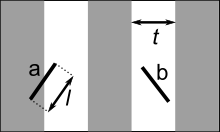
\includegraphics[scale=0.8]{buffon_needle.png}
		\caption{La aguja de Buffon}
		\label{fig:AgujaBuffon}
	\end{figure}
	
	\paragraph{}	
	Los sistemas de simulación de transporte hicieron su aparición hace cuarenta años y la simulación por ordenador comenzó cuando D.L. Gerlough publicó su discurso: \emph{Simulation of freeway traffic on a general-purpose discrete variable computer} (Simulación del tráfico de la autopista en un ordenador de propósito general de variables discretas.) en la Universidad de California, Los Ángeles, en 1955 \cite{Kallberg1971}.
	
	\paragraph{}
	Desde entonces, la simulación por ordenador se ha convertido en una herramienta ampliamente utilizada en la ingeniería del transporte con muchas aplicaciones que van desde la investigación científica hasta la planificación y el entrenamiento.
	
	% Principales líneas de investigación
	
	\paragraph{}
	Actualmente, las líneas de investigación que se están siguiendo en este campo son mayoritariamente simulaciones microscópicas aunque también hay novedades muy interesantes en los modelos teóricos macroscópicos.
	
	% Ejemplo
	
	\paragraph{}
	Como ejemplo de simulador de tráfico podemos nombrar \emph{CORSIM}, el cual permite representar en dos dimensiones una red viaria y simular el flujo del tráfico a lo largo del tiempo indicando una serie de parámetros.
	
	% Integración en el proyecto
	
	\paragraph{}
	En el proyecto que nos ocupa, se va a elaborar un simulador de tráfico microscópico en tres dimensiones que permitirá analizar distintos tipos de configuraciones en una porción limitada de una red viaria.

\newpage

\section{Representación de redes viarias}

	\paragraph{}
	Como se explica en el libro \emph{Fundamentals of Traffic Simulation} \cite{Barcelo2010}, la representación de mapas o de las redes viarias dependerá del tipo de análisis que se quiera llevar a cabo sobre el sistema de transporte.
	
	\paragraph{}
	Inicialmente, la estructura más sencilla para representar lógicamente un mapa será un grafo dirigido, cuyos nodos serán las intersecciones y cuyos arcos serán las secciones viarias que conectan dichas intersecciones, indicando la dirección de las mismas.
	
	\paragraph{}
	Para completar este modelo, se caracterizan los arcos del grafo con atributos como, por ejemplo,  \emph{capacidad del enlace, número de carriles, modos de transporte que pueden utilizar cada carril (bus, coche, taxi, etc), densidad del tráfico, etc.}
	
	\paragraph{}
	Este modelo sencillo puede ser detallado añadiendo nodos para indicar los posibles giros permitidos en una intersección, tal y como se muestra en la figura \ref{fig:RepresentacionMapas1}.
	
	\begin{figure}[ht]
		\centering
			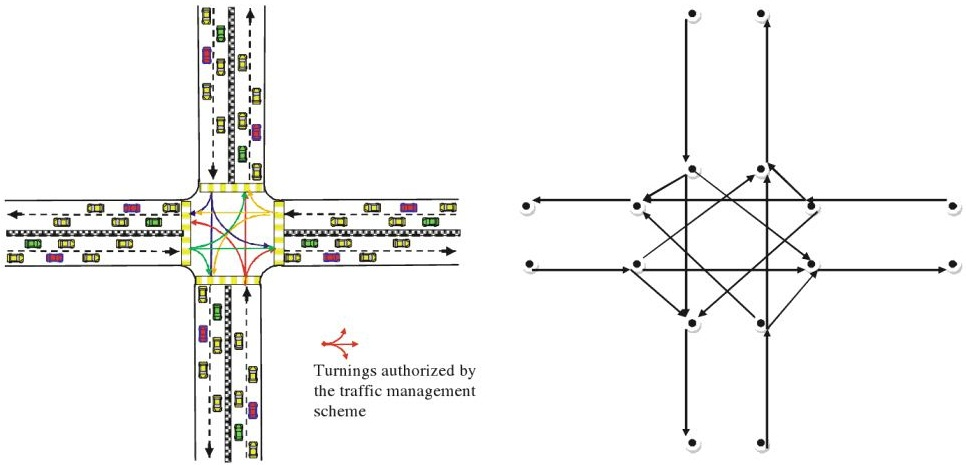
\includegraphics[scale=0.4]{RepresentacionMapas1.jpg}
		\caption{Representación de una intersección (Barceló 2010) \cite{Barcelo2010}}
		\label{fig:RepresentacionMapas1}
	\end{figure}	

	\paragraph{}
	Una vez que tenemos un modelo sencillo, al cual se le pueden añadir tantos detalles como deseemos en forma de atributos en los nodos y en los arcos, se nos presenta el problema de la búsqueda de caminos en una red viaria.
	
	\paragraph{}
	Como solución a dicho problema aparece el estudio \emph{A new data structure to represent road networks} \cite{Bogaert}, en el cual se propone utilizar tres niveles de detalle para representar el mapa. Estos niveles pueden observarse en la figura \ref{fig:RepresentacionMapas2} y en la tabla \ref{table:TablaNiveles}
	
	\begin{figure}[ht]
		\centering
			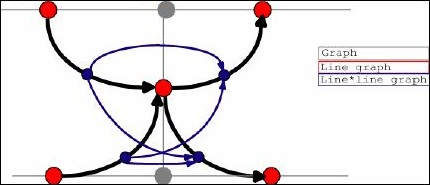
\includegraphics[scale=0.8]{RepresentacionMapas2.jpg}
		\caption{Representación de una intersección (Bogaert) \cite{Bogaert}}
		\label{fig:RepresentacionMapas2}
	\end{figure}
	
	\begin{table}[ht]
		\begin{tabular}{|c|c|c|}
			\hline
			Nivel & Nodos & Arcos \\
			\hline
			\hline
			0 (un grafo) & Intersecciones & Segmentos de vía \\
			\hline
			1 (grafo de líneas) & Segmentos de vía & Giros \\
			\hline
			2 (grafo de líneas de líneas) & Giros & Conexiones entre giros \\
			\hline
		\end{tabular}

	\caption{Niveles representados en la figura \ref{fig:RepresentacionMapas2}}
	\label{table:TablaNiveles}
	\end{table}
	
\section{Sistemas de partículas conductistas}
	
	\paragraph{}
	Los sistemas de partículas son colecciones de objetos independientes, a menudo representados por una sola forma o punto. Todas las partículas tienen una serie de atributos los cuales permiten tener distintos tipos de partícula, tanto en aspecto como en comportamiento.
	
	\paragraph{}
	Generalmente, la implementación de sistemas de partículas conductictas se lleva a cabo mediante la utilización de máquinas de estados finitos, las cuales sirven para modelar el comportamiento de las partículas, de manera que éstas actuarán de una forma u otra en base a sus atributos.
	
	\paragraph{}
	En el caso particular de este proyecto, cada vehículo será una partícula con una serie de características o atributos, lo que nos permitirá modelar distintos tipos de vehículo y distintos tipos de comportamiento de los conductores, con el fin de representar la variedad de los mismos que podemos observar en la realidad.

\section{Modelos de redes viarias reales a partir de imágenes}

	\paragraph{}
	La obtención de redes viarias a partir de imágenes de satélite es un campo de investigación muy importante debido a la gran cantidad de aplicaciones en las que se puede utilizar (militares, civiles, científicas, etc).
	
	\paragraph{}
	El problema consiste en detectar en una imagen, qué es una carretera (camino o vía) y qué no lo es, de forma que esta información pueda ser extraída y procesada.
	
	\paragraph{}
	En el artículo \emph{Road network extraction and intersection detection from aerial images by tracking road footprints} \cite{JiuxiangHu2007} se describe un método de extracción de redes viarias que proporciona muy buenos resultados.
	
	\paragraph{}
	Este método consta de tres pasos:
	\begin{enumerate}	
	\item \emph{Automatic road seeding}: Se analiza el vecindario de todos los píxeles de la imagen y se decide si el pixel es un punto de inicio válido para un segmento de carretera.
	\item \emph{Road tracking}: Comenzando a partir de todas las semillas, se extienden los segmentos de carretera, iterativamente, en una, dos o más direcciones. Se analizan iterativamente el vecindario local de todos los puntos activos en la red viaria para decidir si parar, continuar en una dirección, o dividir en dos o tres direcciones. Este algoritmo va creando un árbol de carreteras.
	\item \emph{Road tree prunning}: Los pasos previos producen una red viaria que contiene casi todos los segmentos de carretera, pero sufre de sobreextracción y pérdidas. Los autores del artículo utilizan una regla de decisión bayesiana para eliminar trozos de la red extraída que parezcan no ser carreteras.
	\end{enumerate}
	
	\paragraph{}
	La inclusión de este método en el proyecto posibilitaría incluir redes viarias reales a la simulación, lo que permitiría probar distintas soluciones de ordenación viaria en entornos reales.

\section{Herramientas gráficas}

	\paragraph{}
	En el apartado gráfico vamos a contar con dos herramientas que se están utilizando mucho en estos tiempos en el área de la informática gráfica. Por un lado podremos usar Unity3D \cite{Unity_web}, que es un motor gráfico de videojuegos, ya que sus características nos permiten simular un sistema de partículas conductista en un entorno 3D sin mucha dificultad. Por otro lado podremos contar con la herramienta Blender \cite{Blender_web}, que se usa en modelado, y nos permitirá incluir los modelos necesarios en la aplicación. Además, esta última se integra perfectamente con la primera.